\section{A Unified Language}

\newcommand\semp[1]{[\![{#1}]\!]}
\newcommand\fix{\operatorname{fix}}

We first set up a formal language that we will use to describe computations and reason about them.
Bellmania uses the same language for specifications and for programs.  Its core is the polymorphic
$\lambda$-calculus, that is, simply typed $\lambda$-calculus with universally quantified type variables 
(also known as \newterm{System F}).

We write abstraction terms as $(v:\T)\mapsto e$, where $\T$ is the type of the argument $v$ and $e$ is
the body. Curried functions $(v_1:\T_1)\mapsto (v_2:\T_2) \mapsto \cdots \mapsto (v_n:\T_n) \mapsto e$ are abbreviated 
as $(v_1:\T_1)\cdots(v_n:\T_n)\mapsto e$.

The semantics differ slightly from that of traditional functional languages: arrow types $\T_1\to\T_2$
are interpreted as {\bf mappings} from values of type $\T_1$ to values of type $\T_2$. Algebraically,
interpretations of types, $\semp{\T_1}$, $\semp{\T_2}$, are sets, and interpretations of arrow-typed terms,
$f : \T_1\to\T_2$, are {\bf partial functions} --- $\semp{f} : \semp{\T_1}\rightharpoonup\semp{\T_2}$.
This implies that a term $t : \T$ may evaluate to an \newterm{undefined} value, $\semp{t}=\bot_\T$
(We would shorten it to $\semp{t}=\bot$ when the type is either insignificant or understood from the context).
For simplicity, we shall identify $\bot_{\T_1\to\T_2}$ with the empty mapping $(v:\T_1)\mapsto\bot_{\T_2}$.

All functions are naturally extended, so that $f\,\bot=\bot$.

\subsection{Operators}
\label{lang:operators}

The core is augmented with the following intrinsic operators:

\begin{itemize}
  \item A fixed point operator $\fix f$, with the denotational semantics
    \[\semp{\fix f} ~=~ \sigma x.~ (\semp f\,x=x)\]
  we assume that recurrences given in specifications are well-defined, 
  such that $\semp f$ has a single fixed point.
  In other words, we ignore nonterminating computations.
  \item A slash operator $/$,
  \[\begin{array}{ll}
      \mbox{For base type $\S$, $x,y:\S$} & x/y = \begin{cases}x & \mbox{if }x\neq\bot \\ y & \mbox{if }x=\bot\end{cases} \\
      \mbox{For $f,g:\T_1\to\T_2$} & f/g = (v:\T_1)\mapsto (f\,v)/(g\,v)
    \end{array}\]
\end{itemize}

\subsection{Types and Type Qualifiers}

We extend the type system with predicate abstraction in the form of logically qualified data types 
(Liquid Types~\cite{PLDI08/Rondon}). These are refinement types restricted via a set of abstraction predicates,
called \newterm{qualifiers}, which are defined over the base types.
Contradictory to the general use of refinement types, the purpose of these qualifiers is not to
check a program for safety and reject ill-typed program, but rather to serve as annotations for
tactics, to convey information to the solver for use in the proof, and later to help the compiler
to properly schedule parallel computations.

As such, we define a Bellmania program to be well-typed iff it is well-typed
without the annotations (in its \newterm{raw form}). Qualifiers are processed
as a separate pass to properly annotate sub-terms.

Some qualifiers are built-in, and more can defined by the user. To keep the syntax simple, we somewhat
limit the use of qualifiers, allowing only the following forms:

\begin{itemize}
  \item $\{v:\T ~|~ P(v)\}$, abbreviated as $\T\cap P$. When the signature of $P$ is known (which is
  almost always), it is enough to write $P$.
  \item $\{v:\T ~|~ P(v)\land Q(v)\}$, abbreviated as $\T\cap P\cap Q$, or just $P\cap Q$. This extends
  to any number of conjuncts of the same form.
  \item $x : \T_2 \to \{v:\T_2 ~|~ R(x,v)\} \to \T_3$, abbreviated as $\big((\T_1\times\T_2)\cap R\big)\to\T_3$.
  The qualifier $R$ must be the preceding argument; this extends to predicates of
  any arity (that is, a $k$-ary predicate in a qualifier is applied to the $k$
  arguments to the left of it, including the current one).
\end{itemize}


\medskip  
The type refinement operators $\cap$ and $\times$ may be composed to create \newterm{droplets},
using the abstract syntax in \Cref{lang:droplets}.
Note that the language does not define tuple types; hence there is no distinction between curried and uncurried function types.
Droplets can express conjunctions of qualifiers,
as long as their argument sets are either disjoint or contained, but not overlapping;
for example, \[x:\{v:\T_1~|~P(v)\}\to \{v:\T_2~|~Q(v)\land R(x,v)\}\to\T_3\] can be written as
$\big((P\times Q)\cap R\big)\to\T_3$, but \[x:\T_1\to y:\{v:\T_2~|~R(x,v)\} \to \{v:\T_3~|~R(y,v)\}\to\T_4\]
cannot be represented as a droplet.

As with any refinement type system, we define the \newterm{shape} of a droplet to be the raw type
obtained from it by removing all qualifiers.

\newcommand\examplePar{%
\noindent\hspace{-2pt}%
\tikz[baseline=(E.base)]\node(E)[draw,rectangle,rounded corners=.7em] {\bf Example};}
\examplePar
The inputs $w$, $w'$ to the Simplified Arbiter (\Cref{intro:arbiter spec}) can be typed using these droplets:
\[
\begin{array}{l}
  w : ((I\times I)\cap{<})\to J\to\R \\
  w' : ((J\times J)\cap{<})\to I\to\R
\end{array}
\]

This states that $w\,p\,i\,j$ is only defined for $p<i$. It doesn't {\em force} it to be defined,
as it is still a partial function. This property is in fact useful: we now have a mechanism for
specifying that some schedules are impossible!

\subsubsection*{Typing Rules}

\begin{figure}
\[
\begin{array}{lcll}
  d       & ::= & e^1 \quad |\quad e^k\to d \\
  e^1     & ::= & \T & \mbox{\it\small for base type $\T$} \\
  e^{k+l} & ::= & e^k \times e^l \\
  e^k     & ::= & e^k \cap P & \mbox{\it\small for $k$-ary predicate symbol $P$} 
\end{array}
\]
\caption{\label{lang:droplets}
  Syntax of type qualifiers (droplets). $k$, $l$ are positive integer
  dimension indexes.}
\end{figure}

As mentioned earlier, annotations are ignored when typechecking a term.
This gives a simple characteristic of type safety without the need to
explictly write any new typing rules. It also means that for $f:\T_1\to\T_2$, $x:T_3$, we obtain $f\,x:\T_2$ whenever
$\T_1$ and $\T_3$ have the same shape. This requires some explanation.

Considering a (partial) function $\T\to\S$ to be a set of pairs of elements $\langle x,y\rangle$ 
from its domain $\T$ and range $\S$, respectively, it is clear to see that any function of type $\T_1\to\S_1$,
such that $\semp{\T_1}\subseteq\semp{\T}$, $\semp{\S_1}\subseteq\semp{\S}$, 
is \emph{also}, by definition, a function of type $\T\to\S$, since $\semp{\T_1}\times\semp{\S_1}\subseteq\semp{\T}\times\semp{\S}$.
If we define subtyping as inclusion of the domains, i.e. $\T_1 <:\T$ whenever $\semp{\T_1}\subseteq\semp{\T}$,
this translates into:
%
\[\T_1<:\T ~\land~ \S_1<:\S ~~\Rightarrow~~ (\T_1\to\S_1) <: (\T\to\S)\]

In this case, the type constructor $\to$ is {\bf covariant} in both arguments.\footnote{This is different from classical view, and holds in this case because we interpret functions as \emph{mappings}.}
With this in mind, a function $g:(\T\to\S)\to \S_2$ can be called with an argument $a: \T_1\to\S_1$,
by regular subtyping rules, and $g\,a : \S_2$.

When the argument's type is not a subtype, but has the same shape as that of the expected type,
it is \newterm{coerced} to the required type by restricting the values to the desired proper subset.
%
\[\mbox{For }h:\T\to\S \qquad \semp{h\,a} ~=~ \semp{h}\big(\semp{a} :: \T\big)\]

Where $::$ is defined as follows:
\begin{itemize}
  \item For scalar (non-arrow) type $\T$, \[x :: \T ~=~ \begin{cases}x & \mbox{if }x\in\semp{\T} \\ \bot & \mbox{if }x\not\in\semp{\T}\end{cases}\]
  \item $f :: \T\to\S ~=~ x\mapsto \big(f\,(x :: \T)\big) :: \S$
\end{itemize}

\medskip
We extend our abstract syntax with an explicit \newterm{cast operator}
$t::\T$ following this semantics.

\subsubsection*{Type Inference}

Base types are inferred normally as in a classical Hindley-Milner type system.
The operators (\Cref{lang:operators}) behave like polymorphic
constants with the following types:
\[\renewcommand\arraystretch{1.5}
  \begin{array}{c}
    {\fix} : (\T\to\T)\to\T \qquad {/} : \T\to\T\to\T \\
    (::\T) : \mathrm{shape}[\T]\to\mathrm{shape}[\T]
  \end{array}\]


Qualifiers are also inferred by essentially propagating them up and down the syntax tree.
Since the program already typechecks once the base types are in place, the problem is no longer
one of finding {\em valid} annotations, but rather of {\em tightening} them as much as possible
without introducing semantics-changing coercions. For example, $(f :: I\to(I\cap P))\,i$ may
be assigned the type $I$, but it can also be assigned $I\cap P$ without changing its semantics.

Qualifiers are propagated by defining a \newterm{type intersection} operator $\sqcap$ that
takes two droplets of the same shape $\T_1$, $\T_2$ and returns a droplet with a conjunction of all the qualifiers
occuring in either $\T_1$ or $\T_2$. The operator is defined in terms of the corresponding liquid types:
\begin{itemize}
  \item If $\T_1=\{v:\T ~|~ \varphi_1\}$ and $\T_2=\{v:\T ~|~ \varphi_2\}$,
	\[\T_1\sqcap\T_2 ~=~ \{v:\T ~|~ \varphi_1\land\varphi_2\}\]
  \item If $\T_1=x:\S_1\to\S_2$, $\T_2=x:\S_3\to\S_4$ (named arguments are normalized so that $\T_1$ and $\T_2$ use the same names),
    \[\T_1\sqcap\T_2 ~=~ x:(\S_1\sqcap\S_3)\to(\S_2\sqcap\S_4)\]
\end{itemize}

We then define the \newterm{type refinement} steps for $e$ a sub-term, listed in \Cref{lang:type refinement rules}.
These rules are applied continuously until a fixed point is reached.
The resulting types are eventually converted back to droplet form (expressed via $\cap$ and $\times$);
qualifiers that cannot be expressed in droplets are discarded.

\begin{figure*}
\newcommand\typerule[2]{{\renewcommand\arraystretch{1.5}\begin{array}[t]{c} #1 \\ \hline #2 \end{array}}}
\[
\renewcommand\arraystretch{4}
\begin{array}{cccp{1cm}}
  \multirow{2}{1cm}[-3em]{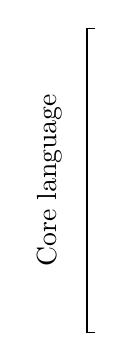
\begin{tikzpicture}\draw (1mm,6em) -- (0,6em) -- (0,-5em) node[midway,above,xshift=-2mm,rotate=90] {Core language} -- +(1mm,0);\end{tikzpicture}} &
  \typerule{e=v \qquad \Gamma,v:\T_1\vdash e:\T_0}
           {\Gamma,v:\T_1 ~\vdash~ e:\T_0\sqcap\T_1} &
  \typerule{e=e_1\,e_2 \qquad \Gamma \vdash e:\T, ~ e_1:\T_1, ~ e_2:\T_2\to\S_2}
           {\renewcommand\arraystretch{1.2}
            \begin{array}[t]{@{}l@{}l@{}}
              \Gamma ~\vdash~ & e:\T\sqcap\S_2, \\ 
                              & e_1:\T_1\sqcap\T_2, \\
                              & e_2:(\T\to\T_1)\sqcap(\T_2\to\S_2)
            \end{array}} & \\
  &
  \cspan2{
  \typerule{e=(v:\T)\mapsto e_1 \qquad \Gamma\vdash e:\T_0\to\S_0 \qquad \Gamma,v:\T\sqcap\T_0\vdash e_1:\T_1}
           {\renewcommand\arraystretch{1.2}
            \begin{array}[t]{r@{}l}
              \Gamma ~\vdash~ & e:(\T_0\to\S_0)\sqcap(\T\to\T_1)\\
              \Gamma,v:\T\sqcap\T_0 ~\vdash~ & e_1:\T_1\sqcap\S_0 
            \end{array}}  } & \\
  %
  \multirow{2}{1cm}[-2.5em]{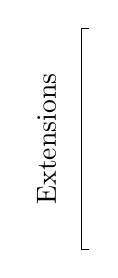
\begin{tikzpicture}\draw (1mm,0) -- (0,0) -- (0,-8em) node[midway,above,xshift=-2mm,rotate=90] {Extensions} -- +(1mm,0);\end{tikzpicture}} &
  \typerule{e=\fix e_1 \qquad \Gamma\vdash e:\T, ~ e_1:\T_1\to\T_2}          % fix
           {\Gamma\vdash e: \T\sqcap\T_2} &
  \typerule{e=e_1/e_2 \qquad \Gamma\vdash e:\T, ~ e_1:\T_1, ~ e_2:\T_2}      % /
           {\renewcommand\arraystretch{1.2}
            \begin{array}[t]{@{}l@{}l@{}}
              \Gamma\vdash{} & e_1:\T_1\sqcap\T \\ & 
                               e_2:\T_2\sqcap\T
            \end{array}} & \\
  &
  \cspan2{
  \typerule{e=e_1::\T \qquad \Gamma\vdash e_1:\T_1}                           % ::
           {\Gamma\vdash e:\T\sqcap\T_1, ~ e_1:\T\sqcap\T_1} } &
\end{array}
\]
\caption{\label{lang:type refinement rules}
  Type refinement rules, for inferring qualifiers in sub-expressions.}
\end{figure*}

Note that two syntactically identical terms in different sub-trees may be assigned
different types by this method. This is a desirable property, as (some) context information
gets encoded in the type that way.

\examplePar Let $I_0\subseteq I$ be a unary predicate, and $0:T$ a constant.
The expression $f\,(i:I_0)\mapsto f\,i\,i ~/~ 0$ will induce the following type
inferences:

\hspace*{\fill}
\begin{tikzpicture}[node distance=1em]
  \node(farg) {$f$};
  \node(iarg)[right=of farg] {$(i:I_0)$};
  \node(mapsto)[right=of iarg] {$\mapsto$};
  \node(f)[right=of mapsto] {$f$};
  \node(i1)[right=of f] {$i$};
  \node(i2)[right=of i1] {$i$};
  \node(slash)[right=of i2] {$\big/$};
  \node(zero)[right=of slash] {$0$};
  \node(l0)[coordinate,below=1mm of farg] {};
  \node(l1)[coordinate,below=4.5mm of l0] {};
  \node(l2)[coordinate,below=3.5mm of l1] {};
  \node(l3)[coordinate,below=3.5mm of l2] {};
  \def\ytip{2pt}
  \draw (l0 -| farg.west) -- +(0,-\ytip) -| (l0 -| farg.east) node[pos=0.25,below] {\tiny $I\to I\to T$};
  \draw (l0 -| f.west) -- +(0,-\ytip) -| (l0 -| f.east) node[pos=0.5,anchor=north east,inner xsep=0] {\tiny $I_0\to I_0\to T$};
  \draw (l0 -| i1.west) -- +(0,-\ytip) -| (l0 -| i1.east) node[pos=0.25,below] {\tiny $I_0$};
  \draw (l0 -| i2.west) -- +(0,-\ytip) -| (l0 -| i2.east) node[pos=0.25,below] {\tiny $I_0$};
  \draw (l0 -| zero.west) -- +(0,-\ytip) -| (l0 -| zero.east) node[pos=0.25,below] {\tiny $T$};
  \draw (l1 -| f.west) -- +(0,-\ytip) -| (l1 -| i1.east) node[pos=0.25,below] {\tiny $I_0\to T$};
  \draw (l2 -| f.west) -- +(0,-\ytip) -| (l2 -| i2.east) node[pos=0.25,below] {\tiny $T$};
  \draw (l3 -| f.west) -- +(0,-\ytip) -| (l3 -| zero.east) node[pos=0.25,below] {\tiny $T$};
\end{tikzpicture}
\hspace*{\fill}

\subsection{Additional Notation}
\newcommand\applt{\textrm{{\scriptsize\,}\guillemotright{\scriptsize\,}}}

We also adopt some syntactic sugar to make complex terms more managable:

\begin{itemize}
  \item $x \applt f ~=~ f\,x$ for application from the left.
  \item $t\big|_{\square}$ abbreviates $t::\square\to\_\,$, where ``$\_$'' is a fresh type variable
    to be inferred. As a special case, $\big|$ can also be applied
    to scalar (non-arrow) expressions by supplying a Boolean condition,
    interpreted as a (nullary) qualifier:
    \[x\big|_{C} ~=~ x :: (\_\cap C) ~=~ \begin{cases}x & \mbox{if }C \\ \bot & \mbox{if }\lnot C\end{cases}\]
\end{itemize}

\subsection{Primitives}

The standard library contains some common primitives:

\begin{itemize}
  \item $\R$, a type for real numbers; $\N$ for natural numbers; $\B$ for Boolean true/false.
  \item ${=} : \T\to\T\to\B$, always interpreted as equality.
  \item ${+}, {-} : \T\to\T\to\T$, polymorphic binary operators.
  \item ${<} : \T\to\T\to\B$, a polymorphic order relation.
  \item $\min, \max, \Sigma : (\T\to\S)\to\S$, reduction (aggregation) operators
    on ordered/unordered collections. The collection is represented by a mapping $f : \T\to\S$,
    so that e.g. \[\semp{\min f} = \min \big\{\semp{f}\,v \;\big|\; v\in\semp{\T}, \semp{f}\,v\neq\bot\big\}\]
    The collections are expected to be finite.
\end{itemize}

\exampleTitle  \begin{comment}\subsection{Example}\end{comment}

\noindent
The specification of the Simplified Gap (\Cref{intro:arbiter spec}) will be written as
%
\begin{equation}
  \renewcommand\arraystretch{1.5}
  \begin{array}{@{}l@{}l@{}l@{}}
    \lspan3{w : ((I\times I)\cap{<})\to J\to\R} \\
    \lspan3{w' : ((J\times J)\cap{<})\to I\to\R} \\
    G ~=~ \fix \theta\,i\,j\mapsto{}
      & \lspan2{0\big|_{i=0\land j=0} ~\Big/~ w'_{0j0}\big|_{i=0} ~\Big/~ w_{0i0}\big|_{j=0} ~\Big/~} \\
      & \min~\langle~ & \min p\mapsto\theta_{pj}+w_{pij}, \\
      & & \min q\mapsto\theta_{iq}+w'_{qji} ~\rangle
  \end{array}
  \label{lang:arbiter spec}
\end{equation}

\medskip
We are using $f_{xy}$
as a more readable alternative typography for $f\,x\,y$,
where $f$ is a function symbol and $x$, $y$ are its arguments.

Note that the ranges for $\min p$ and $\min q$ are implicit, from the types of
$w$, $w'$: \[w_{pij}\neq\bot\limplies p<i \quad \mbox{and} \quad w_{qji}\neq\bot\limplies q<j\]

\medskip
\hrule
